\documentclass[tikz,border=10pt]{standalone}
\usepackage{tikz}
\usetikzlibrary{shapes,arrows,positioning,shadows,fit,calc}

\begin{document}

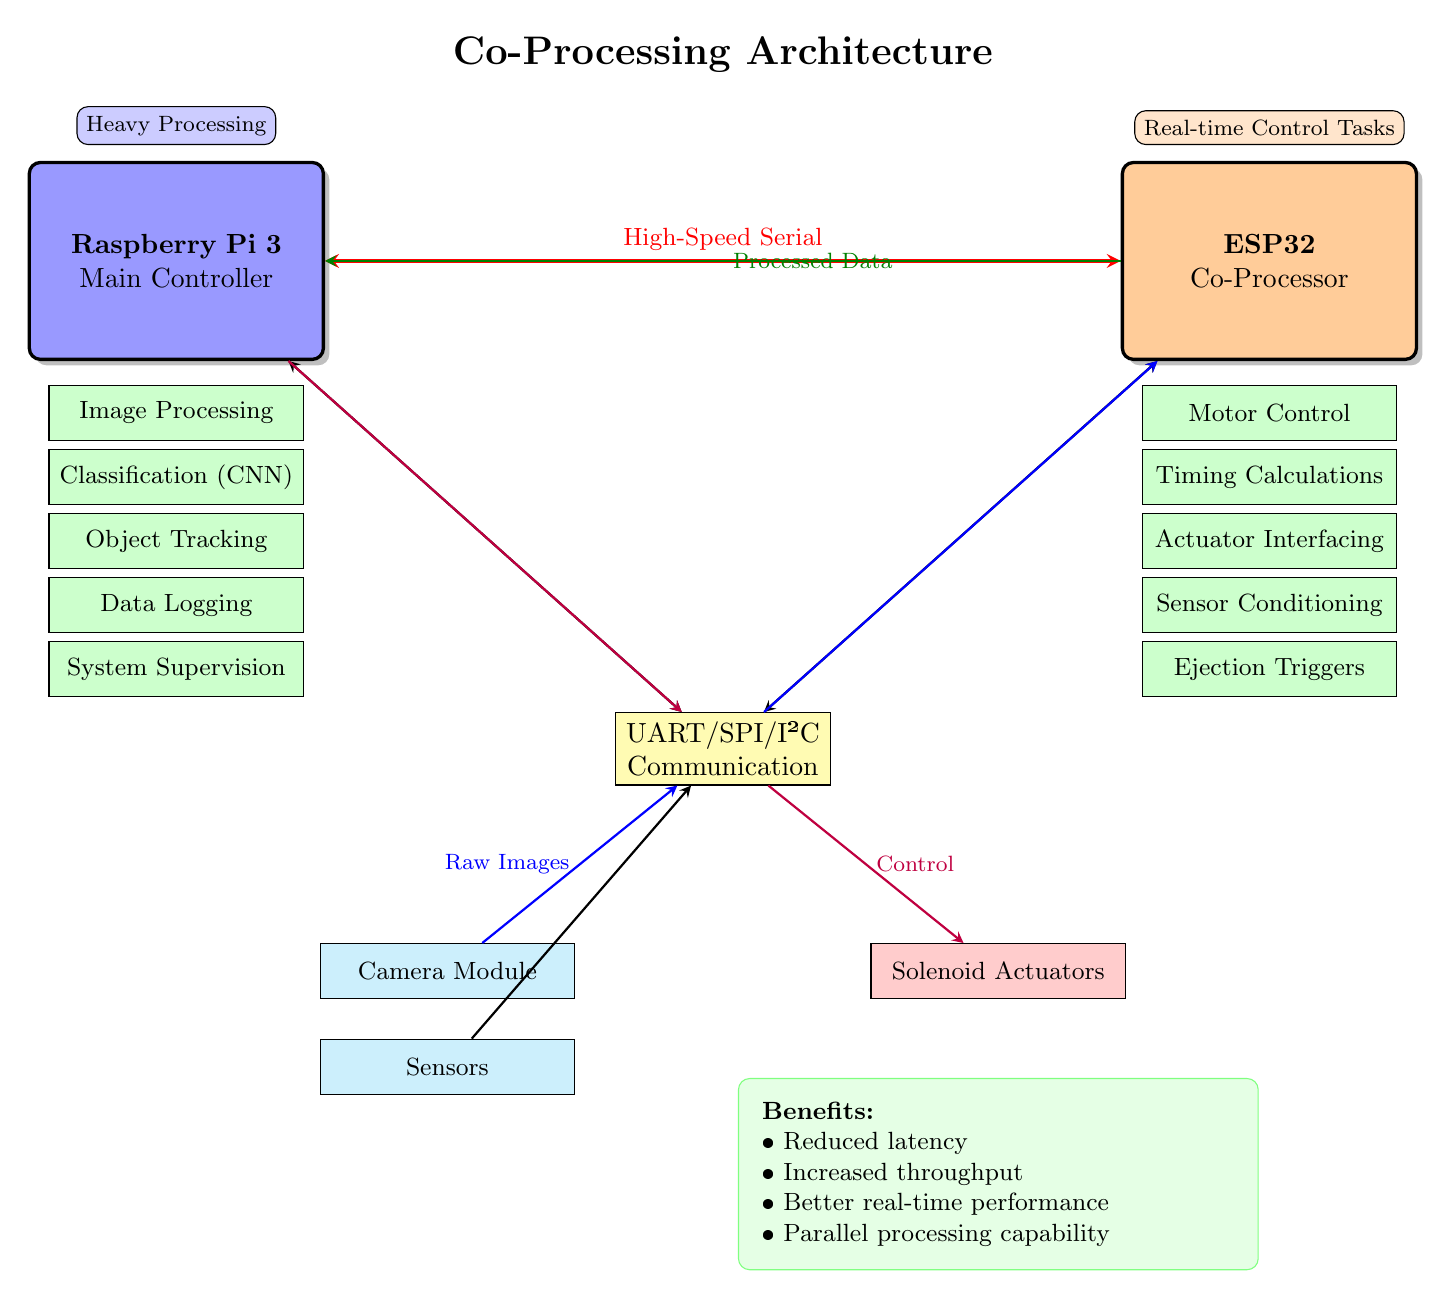
\begin{tikzpicture}[
    node distance=1.2cm,
    processor/.style={rectangle, draw, fill=blue!40, text width=3.5cm, text centered, rounded corners, minimum height=2.5cm, drop shadow, very thick},
    task/.style={rectangle, draw, fill=green!20, text width=3cm, text centered, minimum height=0.7cm, font=\small},
    comm/.style={rectangle, draw, fill=yellow!30, text width=2.5cm, text centered, minimum height=0.8cm},
    arrow/.style={thick,->,>=stealth},
    doublearrow/.style={thick,<->,>=stealth},
    title/.style={font=\bfseries\Large}
]

% Title
\node[title] (title) {Co-Processing Architecture};

% Raspberry Pi 3
\node[processor, below left=1cm and 1.5cm of title] (rpi) {\textbf{Raspberry Pi 3}\\Main Controller};

% Raspberry Pi tasks
\node[task, below=0.3cm of rpi] (rpi1) {Image Processing};
\node[task, below=0.1cm of rpi1] (rpi2) {Classification (CNN)};
\node[task, below=0.1cm of rpi2] (rpi3) {Object Tracking};
\node[task, below=0.1cm of rpi3] (rpi4) {Data Logging};
\node[task, below=0.1cm of rpi4] (rpi5) {System Supervision};

% ESP32/STM32 Co-Processor
\node[processor, below right=1cm and 1.5cm of title, fill=orange!40] (esp) {\textbf{ESP32}\\Co-Processor};

% Co-Processor tasks
\node[task, below=0.3cm of esp] (esp1) {Motor Control};
\node[task, below=0.1cm of esp1] (esp2) {Timing Calculations};
\node[task, below=0.1cm of esp2] (esp3) {Actuator Interfacing};
\node[task, below=0.1cm of esp3] (esp4) {Sensor Conditioning};
\node[task, below=0.1cm of esp4] (esp5) {Ejection Triggers};

% Communication channel
\node[comm, below=8cm of title] (comm) {UART/SPI/I²C\\Communication};

% External components
\node[task, below left=2cm and 0.5cm of comm, fill=cyan!20] (camera) {Camera Module};
\node[task, below right=2cm and 0.5cm of comm, fill=red!20] (actuators) {Solenoid Actuators};
\node[task, below=0.5cm of camera, fill=cyan!20] (sensors) {Sensors};

% Arrows - Communication
\draw[doublearrow, red, very thick] (rpi) -- node[above, sloped, font=\small] {High-Speed Serial} (esp);
\draw[doublearrow] (rpi) -- (comm);
\draw[doublearrow] (esp) -- (comm);

% Arrows - Camera to Co-Processor
\draw[arrow, blue] (camera) -- node[left, font=\footnotesize] {Raw Images} (comm);
\draw[arrow, blue] (comm) -- (esp);

% Arrows - Co-Processor to RPi
\draw[arrow, green!50!black] (esp) -- node[right, font=\footnotesize] {Processed Data} (rpi);

% Arrows - RPi to Actuators
\draw[arrow, purple] (rpi) -- (comm);
\draw[arrow, purple] (comm) -- node[right, font=\footnotesize] {Control} (actuators);

% Arrows - Sensors
\draw[arrow] (sensors) -- (comm);

% Processing load indicators
\node[above=0.2cm of rpi, fill=blue!20, draw, rounded corners, font=\footnotesize] (load1) {Heavy Processing};
\node[above=0.2cm of esp, fill=orange!20, draw, rounded corners, font=\footnotesize] (load2) {Real-time Control Tasks};

% Benefits box
\node[below=1cm of actuators, text width=6cm, fill=green!10, draw=green!50, rounded corners, inner sep=0.3cm, font=\small] (benefits) {
    \textbf{Benefits:}\\
    • Reduced latency\\
    • Increased throughput\\
    • Better real-time performance\\
    • Parallel processing capability
};

\end{tikzpicture}

\end{document}
